\documentclass{article}
\usepackage[utf8]{inputenc}
\usepackage[letterpaper]{geometry}
\usepackage{amsmath}
\usepackage{bm}
\usepackage{algorithm}
\usepackage{algorithmic}
\usepackage{graphicx}
\usepackage{subcaption}

\linespread{1.2}

\title{Numerical Solution of Steady-State Heat Equation}
\author{Jiaqi Li}
\date{November 2018}

\begin{document}

\maketitle

% section on governing equations
\section{Governing Equations}

In this document, we attempt to solve the steady-state heat equation in one- and two- dimensions.
In 1D, we have
\begin{equation} \label{eq:heat_eq1d}
    -kT''(x) = q(x),\quad x \in \Omega
\end{equation}
In 2D, we have
\begin{equation} \label{eq:heat_eq2d}
    -k \nabla^2 T(x,y) = q(x,y),\quad (x,y) \in \Omega
\end{equation}
where $k$ is the thermal conductivity, $T$ is temperature, and $q$ is a given heat source term. $k$
is assumed to be constant throughout the domain. To simplify the problem, we assume $\Omega = (0,1)$ in 1D and 
$\Omega = (0, 1) \times (0, 1)$ in 2D. We further assume Dirichlet boundary condition:
\begin{equation} \label{eq:bc}
    T|_{\partial \Omega} = g
\end{equation}
where $\partial \Omega$ denotes the boundary of domain $\Omega$, and $g$ is a given function defined on $\partial \Omega$. From PDE theory we know that the combination of equation (\ref{eq:heat_eq1d})/(\ref{eq:heat_eq2d}) and (\ref{eq:bc}) forms a well-posed problem provided
that $q$ and $g$ are regular.


% section on discretization schemes
\section{Discretization Schemes}
Central difference is used to discretize the second-order derivative in the heat equation. 

\begin{figure}
    \centering
    \begin{subfigure}{.5\textwidth}
        \centering
        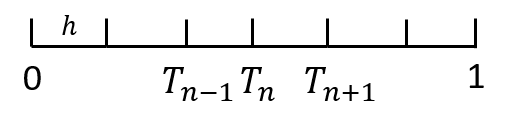
\includegraphics[width=0.9\linewidth]{1d_mesh.png}
        \caption{1D mesh}
    \end{subfigure}%
    \begin{subfigure}{.5\textwidth}
        \centering
        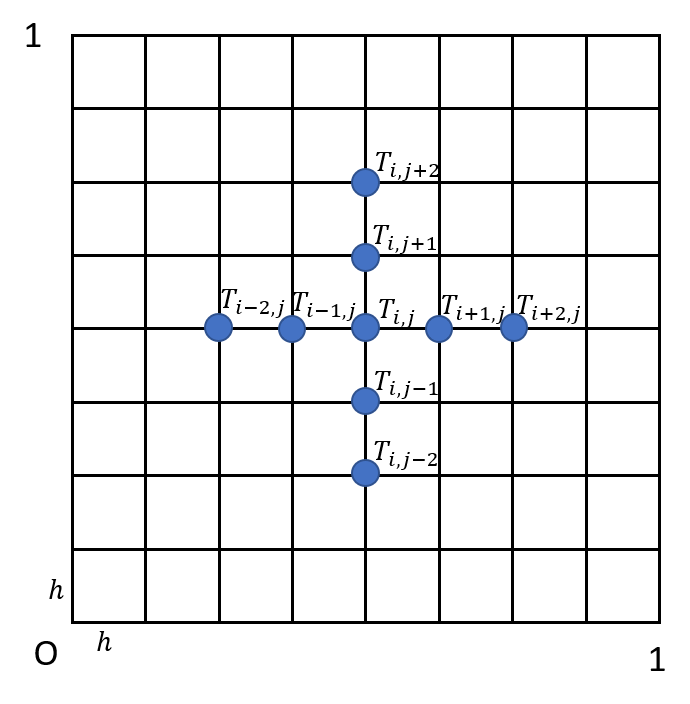
\includegraphics[width=0.9\linewidth]{2d_mesh.png}
        \caption{2D mesh}
    \end{subfigure}
    \caption{Representative figures of 1D and 2D mesh}
\end{figure}

% 1D case
\subsection{1D case}
In 1D case, we partition the domain into uniform intervals. Assume $0 = x_0 < x_1 < ... < x_m = 1$, and $x_n - x_{n-1} = h,\  n = 1, 2, ..., m$.
The second-order approximation to the second-order derivative is
    $$T''(x_n) = \frac{1}{h^2}\left(T_{n-1} - 2 T_n + T_{n+1}\right) + O(h^2)$$
where $T_n = T(x_n)$.
Then the discrete approximation to equation (\ref{eq:heat_eq1d}) is
    $$\frac{1}{h^2}\left(T_{n-1} - 2 T_n + T_{n+1}\right) + O(h^2) = -\frac{q_n}{k}$$
where $q_n = q(x_n)$. In order to get an approximate solution, we neglect the second-order term, and obtain
\begin{equation} \label{eq:heat_eq1d_order2}
    T_{n-1} - 2 T_n + T_{n+1} = -\frac{q_n h^2}{k}, \quad n = 1, 2, ..., m-1
\end{equation}
The boundary condition (\ref{eq:bc}) implies
\begin{equation} \label{eq:bc_order2}
    T_0 = g(0), \quad T_m = g(1)
\end{equation}
Equations (\ref{eq:heat_eq1d_order2}) and (\ref{eq:bc_order2}) form a solvable linear system.

The fourth-order scheme is
    $$T''(x_n) = \frac{1}{h^2}\left( -\frac{1}{12}T_{n-2} + \frac{4}{3}T_{n-1} - \frac{5}{2}T_n + \frac{4}{3}T_{n+1}
    - \frac{1}{12}T_{n+2} \right) + O(h^4)$$
The corresponding discrete approximation to equation (\ref{eq:heat_eq1d}) is
    $$ \frac{1}{h^2}\left( -\frac{1}{12}T_{n-2} + \frac{4}{3}T_{n-1} - \frac{5}{2}T_n + \frac{4}{3}T_{n+1}
    - \frac{1}{12}T_{n+2} \right) + O(h^4) = -\frac{q_n}{k} $$
For practical calculation, we neglect the fourth-order term, obtaining
\begin{equation} \label{eq:heat_eq1d_order4}
     -\frac{1}{12}T_{n-2} + \frac{4}{3}T_{n-1} - \frac{5}{2}T_n + \frac{4}{3}T_{n+1}
    - \frac{1}{12}T_{n+2}  = -\frac{q_n h^2}{k}, \quad n = 2, 3, ..., m-2
\end{equation}
The boundary condition (\ref{eq:bc_order2}) still applies. However, we need two more equations to close the system.
A simple choice is to use second-order difference at the nodes adjacent to the boundary.
\begin{equation} \label{eq:bc_order4}
    T_{n-1} - 2 T_n + T_{n+1} = -\frac{q_n h^2}{k}, \quad n = 1, m-1
\end{equation}
Equations (\ref{eq:heat_eq1d_order4}) together with (\ref{eq:bc_order2}) and (\ref{eq:bc_order4}) form a solvable linear system.

% 2D case
\subsection{2D case}
In 2D case, we partition the domain uniformly in both $x$ and $y$ direction. Let $0 = x_0 < x_1 < ... < x_m = 1$,
and $0 = y_0 < y_1 < ... < y_n = 1$. Let $\Delta x$ and $\Delta y$ be the mesh size in $x$ and $y$ direction, respectively. The second-order approximation to derivatives in the heat equation (\ref{eq:heat_eq2d}) is
\begin{equation*}
\begin{split}
    \nabla^2 T(x_i, y_j) & = \left(\frac{\partial}{\partial x^2} + \frac{\partial}{\partial y^2}\right) T|_{(x_i,y_j)} \\
    & = \frac{1}{\Delta x^2}(T_{i-1,j} - 2T_{i,j} + T_{i+1,j}) + \frac{1}{\Delta y^2}(T_{i,j-1} -2T_{i,j} + T_{i,j+1})
    + O(\Delta x^2) + O(\Delta y^2)
\end{split}
\end{equation*}
The approximation to the equation is
\begin{equation*}
    \frac{1}{\Delta x^2}(T_{i-1,j} - 2T_{i,j} + T_{i+1,j}) + \frac{1}{\Delta y^2}(T_{i,j-1} -2T_{i,j} + T_{i,j+1}) + O(\Delta x^2) + O(\Delta y^2) = - \frac{q_{i,j}}{k}
\end{equation*}
where $q_{i,j} = q(x_i,y_j)$.
When $m = n$, and therefore $\Delta x = \Delta y = h$, the above equation can be simplified as
\begin{equation} \label{eq:heat_eq2d_order2}
    T_{i,j-1} + T_{i-1,j} - 4T_{i,j} + T_{i+1,j} + T_{i,j+1} = - \frac{q_{i,j} h^2}{k},
    \quad i, j = 1, 2, ..., n-1
\end{equation}
where we have omitted the second-order error $O(h^2)$. The boundary condition (\ref{eq:bc}) implies
\begin{equation} \label{eq:bc_2d_order2}
    T_{0,j} = g(0,y_j), \quad T_{n,j} = g(1,y_j), \quad T_{i,0} = g(x_i,0), \quad T_{i,n} = g(x_i, 1)
\end{equation}
for $i = 1, 2, ..., n-1$ and $j = 0, 1, ..., n$. Equations (\ref{eq:heat_eq2d_order2}) and (\ref{eq:bc_2d_order2}) form a closed linear system.

The fourth-order approximation to derivatives is
\begin{equation*}
\begin{split}
    \nabla^2 T(x_i, y_j) = & \frac{1}{\Delta x^2} \left( -\frac{1}{12}T_{i-2,j} + \frac{4}{3}T_{i-1,j}
    - \frac{5}{2}T_{i,j} + \frac{4}{3}T_{i+1,j} - \frac{1}{12}T_{i+2,j} \right) + O(\Delta x^4) \\
    + & \frac{1}{\Delta y^2} \left( -\frac{1}{12}T_{i,j-2} + \frac{4}{3}T_{i,j-1} - \frac{5}{2}T_{i,j}
    + \frac{4}{3}T_{i,j+1} - \frac{1}{12}T_{i,j+2} \right) + O(\Delta y^4)
\end{split}
\end{equation*}
The approximation to the heat equation (\ref{eq:heat_eq2d}) is
\begin{equation*}
\begin{split}
    & \frac{1}{\Delta x^2} \left( -\frac{1}{12}T_{i-2,j} + \frac{4}{3}T_{i-1,j}
    - \frac{5}{2}T_{i,j} + \frac{4}{3}T_{i+1,j} - \frac{1}{12}T_{i+2,j} \right) + O(\Delta x^4) \\
    + & \frac{1}{\Delta y^2} \left( -\frac{1}{12}T_{i,j-2} + \frac{4}{3}T_{i,j-1} - \frac{5}{2}T_{i,j}
    + \frac{4}{3}T_{i,j+1} - \frac{1}{12}T_{i,j+2} \right) + O(\Delta y^4)
    = - \frac{q_{i,j}}{k}
\end{split}
\end{equation*}
Assume $m = n, \Delta x = \Delta y = h$. Then the above equation can be simplified:
\begin{multline} \label{eq:heat_eq2d_order4}
    -\frac{1}{12}T_{i,j-2} + \frac{4}{3}T_{i,j-1} - \frac{1}{12}T_{i-2,j} + \frac{4}{3}T_{i-1,j}
    - 5T_{i,j} \\
    + \frac{4}{3}T_{i+1,j} - \frac{1}{12}T_{i+2,j} + \frac{4}{3}T_{i,j+1} - \frac{1}{12}T_{i,j+2}
    = - \frac{q_{i,j} h^2}{k}
\end{multline}
for $i,j = 2, 3, ..., n-2$, where we have omitted the fourth-order error $O(h^4)$. The boundary condition
(\ref{eq:bc_2d_order2}) still holds, but we need $(4n - 8)$ more equations to close the system. A simple
choice is to use second-order difference at the nodes adjacent to the boundary:
\begin{equation} \label{eq:bc_2d_order4}
    T_{i,j-1} + T_{i-1,j} - 4T_{i,j} + T_{i+1,j} + T_{i,j+1} = - \frac{q_{i,j} h^2}{k}
\end{equation}
where $1 \le i,j \le n-1$ and at least one of $i,j$ equals $1$ or $n-1$. Equations (\ref{eq:heat_eq2d_order4})
together with (\ref{eq:bc_2d_order2}) and (\ref{eq:bc_2d_order4}) form a closed linear system.

% section on resulting linear systems and solution method
\section{Implementation}

\subsection{Resulting linear system}
\subsubsection{1D case}
Let $$\bm{u} = \begin{bmatrix} T_0 & T_1 & \dots & T_m \end{bmatrix}^T$$ be a column vector of unknowns.
The second-order finite difference scheme (\ref{eq:heat_eq1d_order2}), (\ref{eq:bc_order2}) gives the 
following tridiagonal linear system
\begin{equation*}
    \begin{bmatrix} 
    1 \\
    1 & -2 &  1 \\
      &  1 & -2     &  1   \\
      &    & \ddots & \ddots & \ddots \\
      &    &        & 1      & -2     &  1 \\
      &    &        &        &        &  1
    \end{bmatrix}
    \begin{bmatrix}
    T_0 \\ T_1 \\ T_2 \\ \vdots \\ T_{m-1} \\ T_m
    \end{bmatrix}
    =
    \begin{bmatrix}
    g(0) \\ -q_1 h^2/k \\ -q_2 h^2/k \\ \vdots \\ -q_{m-1} h^2/k \\ g(1)
    \end{bmatrix}
\end{equation*}
where zeros in the matrix are omitted. There are three non-zero entries on an interior row of the matrix.

The fourth-order difference scheme (\ref{eq:heat_eq1d_order4}), (\ref{eq:bc_order2}), and (\ref{eq:bc_order4}) 
results in the following linear system
\begin{equation*}
    \begin{bmatrix}
    1 \\
    1  & -2  & 1 \\
    -\frac{1}{12} & \frac{4}{3} & -\frac{5}{2} & \frac{4}{3} & -\frac{1}{12} \\
          & \ddots & \ddots & \ddots & \ddots & \ddots \\ 
          &        & -\frac{1}{12} & \frac{4}{3} & -\frac{5}{2} & \frac{4}{3} & -\frac{1}{12} \\
          &        &               &             &   1          &     -2      &     1  \\
          &        &               &             &              &             &     1
    \end{bmatrix}
    \begin{bmatrix}
    T_0 \\ T_1 \\ T_2 \\ \vdots \\ T_{m-2} \\ T_{m-1} \\ T_m
    \end{bmatrix}
    =
    \begin{bmatrix}
    g(0) \\ -q_1 h^2/k \\ -q_2 h^2/k \\ \vdots \\ -q_{m-2}h^2/k \\ -q_{m-1} h^2/k \\ g(1)
    \end{bmatrix}    
\end{equation*}
There are five non-zero entries on an interior row of the matrix.

\subsubsection{2D case}
Assume $m = n$. Let
\begin{equation*}
    \bm\alpha_j =
    \begin{bmatrix}
    T_{0,j} & T_{1,j} & \dots & T_{n,j}
    \end{bmatrix}^T ,
    \quad j = 0, 1, \dots, n
\end{equation*}
The second-order difference scheme (\ref{eq:heat_eq2d_order2}), (\ref{eq:bc_2d_order2}) gives
\begin{equation} \label{eq:block_2d_order2}
    \bm C \bm\alpha_{j-1} + \bm B \bm\alpha_j + \bm C \bm\alpha_{j+1} = \bm f_j,
    \quad j = 1, 2, \dots, n-1
\end{equation}
where
\begin{equation*}
    \bm B = 
    \begin{bmatrix}
    1 \\
    1 & -4 & 1 \\
      & \ddots & \ddots & \ddots \\
      &        & 1      &   -4   &  1 \\
      &        &        &        &  1
    \end{bmatrix},
    \quad
    \bm C =
    \begin{bmatrix}
    0 \\
      &  1  \\
      &     & \ddots \\
      &     &        &  1 \\
      &     &        &    & 0
    \end{bmatrix}
\end{equation*}
are $(n+1) \times (n+1)$ matrices, and
\begin{equation*}
    \bm f_j = 
    \begin{bmatrix}
    T_{0,j} & -q_{1,j} h^2 /k & \dots & -q_{n-1,j}h^2/k & T_{n,j}
    \end{bmatrix}^T
\end{equation*}
is column vector with length ($n+1$). Rewriting equation (\ref{eq:block_2d_order2}) using block matrices,
we obtain
\begin{equation*}
    \begin{bmatrix}
    \bm{I} \\
    \bm C & \bm B & \bm C \\
      & \ddots & \ddots & \ddots \\
      &        & \bm C  &  \bm B & \bm C \\
      &        &        &        & \bm I
    \end{bmatrix}
    \begin{bmatrix}
    \bm\alpha_0 \\ \bm\alpha_1 \\ \vdots \\ \bm\alpha_{n-1} \\ \bm\alpha_n 
    \end{bmatrix}
    =
    \begin{bmatrix}
    \bm\alpha_0 \\ \bm f_1 \\ \vdots \\ \bm f_{n-1} \\ \bm\alpha_n
    \end{bmatrix}
\end{equation*}
Note that $\bm\alpha_0$ and $\bm\alpha_n$ on the right hand side is given by boundary condition
(\ref{eq:bc_2d_order2}). There are five non-zero entries on an interior row of the matrix.

The second-order scheme (\ref{eq:heat_eq2d_order4}), (\ref{eq:bc_2d_order2}), (\ref{eq:bc_2d_order4}) results
in the following equations for $\bm\alpha_j$:
\begin{equation*}
    \bm F \bm\alpha_{j-2} + \bm E \bm\alpha_{j-1} + \bm D \bm\alpha_j + \bm E \bm\alpha_{j+1} 
    + \bm F \bm\alpha_{j+2} = \bm f_j,
    \quad j = 2, 3, ..., n-2
\end{equation*}
where
\begin{equation*}
    \bm D =     \begin{bmatrix}
    1 \\
    1  & -4  & 1 \\
    -\frac{1}{12} & \frac{4}{3} & -5 & \frac{4}{3} & -\frac{1}{12} \\
          & \ddots & \ddots & \ddots & \ddots & \ddots \\ 
          &        & -\frac{1}{12} & \frac{4}{3} & -5 & \frac{4}{3} & -\frac{1}{12} \\
          &        &               &             &   1          &     -4      &     1  \\
          &        &               &             &              &             &     1
    \end{bmatrix}
\end{equation*}
\begin{equation*}
    \bm E = 
    \begin{bmatrix}
    0 \\
      &  1 \\
      &   & \frac{4}{3} \\
      &   &            & \ddots \\
      &   &            &       & \frac{4}{3} \\
      &   &            &       &            & 1 \\
      &   &            &       &            &  & 0
    \end{bmatrix},
    \bm F =
    \begin{bmatrix}
    0 \\
      &  0 \\
      &   & -\frac{1}{12} \\
      &   &            & \ddots \\
      &   &            &       & -\frac{1}{12} \\
      &   &            &       &            & 0 \\
      &   &            &       &            &  & 0
    \end{bmatrix},    
\end{equation*}
are $(n+1) \times (n+1)$ matrices. Then the global system is
\begin{equation*}
    \begin{bmatrix}
    \bm I \\
    \bm C  & \bm B  & \bm C \\
    \bm F  & \bm E  & \bm D & \bm E & \bm F \\
          & \ddots & \ddots & \ddots & \ddots & \ddots \\ 
          &        & \bm F  & \bm E  & \bm D & \bm E & \bm F \\
          &        &               &             &   \bm C  & \bm B  & \bm C \\
          &        &               &             &              &    & \bm I
    \end{bmatrix}
    \begin{bmatrix}
    \bm\alpha_0 \\ \bm\alpha_1 \\ \bm\alpha_2 \\ \vdots \\ \bm\alpha_{n-2} \\ \bm\alpha_{n-1} \\ \bm\alpha_n
    \end{bmatrix}
    =
    \begin{bmatrix}
    \bm\alpha_0 \\ \bm f_1 \\ \bm f_2 \\ \vdots \\ \bm f_{n-2} \\ \bm f_{n-1} \\ \bm\alpha_n
    \end{bmatrix}    
\end{equation*}
There are nine non-zero entries on an interior row of the matrix.

\subsection{Iterative solutions for the resulting linear system}
Once the linear system is formed, we utilize iterative methods to solve the system. Suppose the system is
\begin{equation*}
    \bm{Ax} = \bm b
\end{equation*}
where $\bm A$ is an $n\times n$ matrix.

\subsubsection{Jacobi method}
\begin{algorithm}[H]
\caption{Jacobi iteration}
\begin{algorithmic}
\STATE $\bm x^{(0)} \leftarrow 0$
\FOR{$k = 0, 1, \dots$}
\STATE $$x_i^{(k+1)} \leftarrow \frac{1}{a_{ii}}\left(b_i - \sum_{j\ne i} a_{ij}x_j^{(k)}\right)$$
    \IF{$||\bm x^{(k+1)} - \bm x^{(k)}|| < tol$}
\STATE       \textbf{exit}
    \ENDIF
\ENDFOR
\end{algorithmic}
\end{algorithm}

\subsubsection{Gauss-Seidel method}
\begin{algorithm}[H]
\caption{Gauss-Seidel iteration}
\begin{algorithmic}
\STATE $\bm x^{(0)} \leftarrow 0$
\FOR{$k = 0, 1, \dots$}
\STATE $$x_i^{(k+1)} \leftarrow \frac{1}{a_{ii}}\left(b_i - \sum_{j=1}^{i-1} a_{ij}x_j^{(k+1)}
    - \sum_{j=i+1}^n a_{ij}x_j^{(k)}\right)$$
    \IF{$||\bm x^{(k+1)} - \bm x^{(k)}|| < tol$}
\STATE       \textbf{exit}
    \ENDIF
\ENDFOR
\end{algorithmic}
\end{algorithm}

\subsection{Required memory}
We will need to store two discrete temperature fields and one source term field. Using double precision, in 1D,
the memory required is $24n$ Bytes; in 2D, we need $24n^2$ Bytes. Since we are using iterative methods
to solve the system, the matrix $\bm A$ is never explicitly formed. In order to calculate the 
difference between two iterations, we need keep a copy of $\bm x^{(k)}$ while computing $\bm x^{(k+1)}$.


\end{document}

